% Default mode is landscape, which is what we want, however dvips and
% a0poster do not quite do the right thing, so we end up with text in
% landscape style (wide and short) down a portrait page (narrow and
% long). Printing this onto the a0 printer chops the right hand edge.
% However, 'psnup' can save the day, reorienting the text so that the
% poster prints lengthways down an a0 portrait bounding box.
%
% 'psnup -w85cm -h119cm -f poster_from_dvips.ps poster_in_landscape.ps'

\documentclass[a0]{a0poster}
% You might find the 'draft' option to a0 poster useful if you have
% lots of graphics, because they can take some time to process and
% display. (\documentclass[a0,draft]{a0poster})
\usepackage[latin1]{inputenc}
\pagestyle{empty}
\renewcommand{\d}{\mathrm{d}}
\newcommand{\sgn}[1]{\mathop{\mathrm{sgn}}#1}
\newcommand{\bu}{\mathbf{u}}
\newcommand{\bx}{\mathbf{x}}
\newcommand{\br}{\mathbf{r}}
\newcommand{\ds}{\mathrm{d}s}
\newcommand{\ie}{\textit{i.e.}}
\setcounter{secnumdepth}{0}
\newcommand{\comment}[1]{}

% The textpos package is necessary to position textblocks at arbitary 
% places on the page.
\usepackage[absolute]{textpos}

% Graphics to include graphics. Times is nice on posters, but you
% might want to switch it off and go for CMR fonts.
\usepackage{tikz}
\usepackage{graphics}
\usepackage{wrapfig,helvet}
\usepackage{amsmath}


% These colours are tried and tested for titles and headers. Don't
% over use color!
\usepackage{color}
\definecolor{DarkBlue}{rgb}{0.1,0.1,0.5}
\definecolor{Red}{rgb}{0.9,0.0,0.1}
\definecolor{headingcol}{rgb}{0.5,0.7,1}
%\definecolor{boxcol}{rgb}{0.3,0.8,0.1}

% see documentation for a0poster class for the size options here
\let\Textsize\normalsize
\def\Head#1{\noindent\hbox to \hsize{\hfil{\LARGE\color{DarkBlue}\sf #1}}\bigskip}
\def\LHead#1{\noindent{\LARGE\color{DarkBlue}\sf #1}\bigskip}
\def\Subhead#1{\noindent{\large\color{DarkBlue}\sf #1}\bigskip}
\def\Title#1{\noindent{\VeryHuge\color{Red}\bf\sf #1}}

\TPGrid[40mm,40mm]{23}{12}  % 3 cols of width 7 plus 2 gaps width 1

\parindent=0pt
\parskip=0.5\baselineskip

\makeatletter							%Needed to include code in main file
\renewcommand\@maketitle{%
\null									%Sets position marker
{
\color{headingcol}\sffamily\VERYHuge		%Set title font and colour
\@title \par}%
\vskip 0.6em%
{
\color{white}\sffamily\LARGE				%Set author font and colour
\lineskip .5em%
\begin{tabular}[t]{l}%
\@author
\end{tabular}\par}%
\vskip 1cm
\par
}
\makeatother

\title{Information Retrieval and Data Mining - Project 6}

\author{Shaun Dowling, Alessandro Ialongo, Andrey Levushkin, Matthieu Louis\\ University College London}

\begin{document}
%----------------------------------------------------------------------%
%           Title bar: across all 21 columns                           %
%----------------------------------------------------------------------%
\begin{textblock}{23}(0,0)
\vspace*{-48mm}\hspace*{-42mm}%
\includegraphics{ucl_bar_black.eps}
\begin{minipage}{1191mm}		%Minipage for title contents
\vspace{-20cm}
\maketitle
\end{minipage}
\end{textblock}

%%%%%%%%%%%%%%%%%% Will need to shift all other content down a bit %%%%%

%----------------------------------------------------------------------%
%           First column.                                              %
%----------------------------------------------------------------------%
\begin{textblock}{7}(0,2.4)
\Head{Introduction}

\sf % Selects sans serif family: part of the UCL corporate image!
Trying to predict the direction of stock markets with a certain degree of confidence has always been the dream of all traders. With the massive increase of available data - financial stocks tick data or social media data (facebook, twitter, etc.) for example - there has been a strong interest in developing mathematical models that leverage those in order to predict and profit from price movements.

A recent and popular model involves estimating the sentiment (i.e. the mood) of a relevant live stream of tweets as a predictor of market changes. One assumption the model makes is that stock prices are led by the behaviour of a large group of people and that this behaviour is correlated to the overall mood of that group of person. Another model would be to just look at tweets and pick out the ones which relate to financial news and try to take a position before the whole market has had time to react to that news event.


\bigskip
\hrule
\end{textblock}

\begin{textblock}{7}(0,5)
\Head{Pipeline}
\begin{figure*}
\begin{center}
\includegraphics[scale=1.2]{Graph_IRDM_pipeline}
\end{center}
\caption{A diagram of our pipeline.}
\end{figure*}

\bigskip
\hrule
\end{textblock}

\begin{textblock}{7}(0,8.8)
\Head{Feature Extraction}

\sf
The key objective of this project is to use information contained within Twitter posts to predict the mood of the markets towards certain stocks. 
Tweets contain a great deal of information, links between users, links to entities (either explicitly view a tag or plain text) and network effect via re-tweets.

In their raw form, Tweets are not convenient for inference. As such we will focus a great deal of our time distilling the information contained within the Tweets while ensuring all important aspects are preserved.
This approach gives a nice layer of abstraction between the Information Retrieval and the Machine Learning steps in the pipeline. 
We will be gathering these features using two independent MapReduce jobs.

\Subhead{Global Statistics}

\sf
Firstly, we will run a global job to gather statistics that depend on the entire dataset (for example tf/idf).
The statistics available and the manner in which they are gathered will be a significant area of experimentation.Some statistics that we plan to start with are:
\begin{itemize}
\item user average sentiment - to help us reduce bias from general opinion. This could be global or regarding a specific company.
\item inverse document frequency - to be used with term frequency within tweets to potentially highlight particularly significant phrases
\item cliques of users (strongly connected groups) - experiment with the effect of an entire connected group having a particular sentiment or sudden change of sentiment
\end{itemize}


\end{textblock}

\begin{textblock}{7}(8,2.4)

\Subhead{Extractor}

\sf
Having gathered global statistics, we can split with another map the Tweets by time segment such that the reducer can then create a full feature vector for each time slice as we see fit.
Architecturally, there will be an abstract Extractor component within the reducer that is given the full list of tweets to process.
This component will be the central component of change in order to explore different options in feature extraction.
The Extractor will also have access to whatever global statistics produced previously in order to compute more complex features

\sf
Key local features that initially be calculated will be things like
\begin{itemize}
\item entity mentions - a base feature which will be joined with a number of other to attribute features to the company whose stock we are interested in
\item sentiment - tied to a specific entity or connected group of users
\item word frequencies - again tied to a entity
\item user ID - which users are mentioning a company
\item number of re-tweets - potentially linked to other statistics so that they can be weighted accordingly
\end{itemize}

\bigskip
\hrule


%----------------------------------------------------------------------%
%           Second column.                                             %
%----------------------------------------------------------------------%



\Head{Machine Learning}

\sf
The feature extraction process provides the raw material on which to construct models to explain the data and to formulate predictions about stock prices given new Tweets. In our project we will consider three main statistical models to uncover the patterns in the data:
\begin{itemize}
\item Linear Regression
\item Support Vector Machine (SVM)
\item Gaussian Process
\end{itemize}
Each of these models will make use of a portion of the available Twitter data (between 70\% and 90\% of the data, ordered chronologically) in combination with stock price data to extract the optimal parameters (according to a loss function). The parameterised models will then be used to predict the more recent performance of the relevant stocks given the remaining portion of the Twitter data. These predictions will then be evaluated against the real-world performance. 

\Subhead{Linear Regression}
\\We will use regularised linear regression with the MSE (mean squared error) loss function (ridge regression) to give us a simple baseline on our predictive performance. With this simple model, we hope to find a linear relation (i.e. linear coefficients) between the features previously extracted and the stock prices. The (Tikhonov) regularisation will be parameterised by a lambda value which will determine the extent to which more complex (larger) coefficients will be penalised in our MSE loss function.

\Subhead{SVM}
\\When predicting simple increase or decreases in stock prices (see evaluation), the problem becomes a classification rather than a regression one. Thus we can use a support vector machine (experimenting with possible kernels and respective parameters) to fit a hyperplane in the feature space between the time splits in the Twitter data that corresponded to increases in the relevant stock prices from those that corresponded to decreases. 

\Subhead{Gaussian Process}
\\For the regression task we will also attempt to describe the stock market as a Gaussian interaction of multiple samples defined by a suitable (kernel) covariance matrix. Defining this matrix will allows us to model periodicities, and the decay of correlation between adjacent samples. Out of the three, this model is the most elaborate as it allows for the greatest flexibility on the relation between the features and the stock prices. In fact the kernel covariance can encode very complex nonlinear relations between features and data-points.  This requires also a higher degree of cross-validation to select the most effective kernel and its hyperparameters.

%\begin{figure*}
%\begin{center}
%\includegraphics[scale=1.5]{gaussian_processes}
%\end{center}
%\caption{An example of a Gaussian Process Model.}
%\end{figure*}

\bigskip
\hrule
\end{textblock}

%----------------------------------------------------------------------%
%           Third column.                                              %
%----------------------------------------------------------------------%
\begin{textblock}{7}(16,2.4)

\Head{Performance Evaluation}

\Subhead{ML algorithm performance}

\sf
To demonstrate the effectiveness of our learning algorithms we proceed by splitting the data into testing and training sets. Than we predict the future stock price using the training set and compute the mean squared error of the prediction using the test set. An example of discrepancy between the predicted and actual price that we hope to minimise is shown below.

\begin{figure*}
\begin{center}
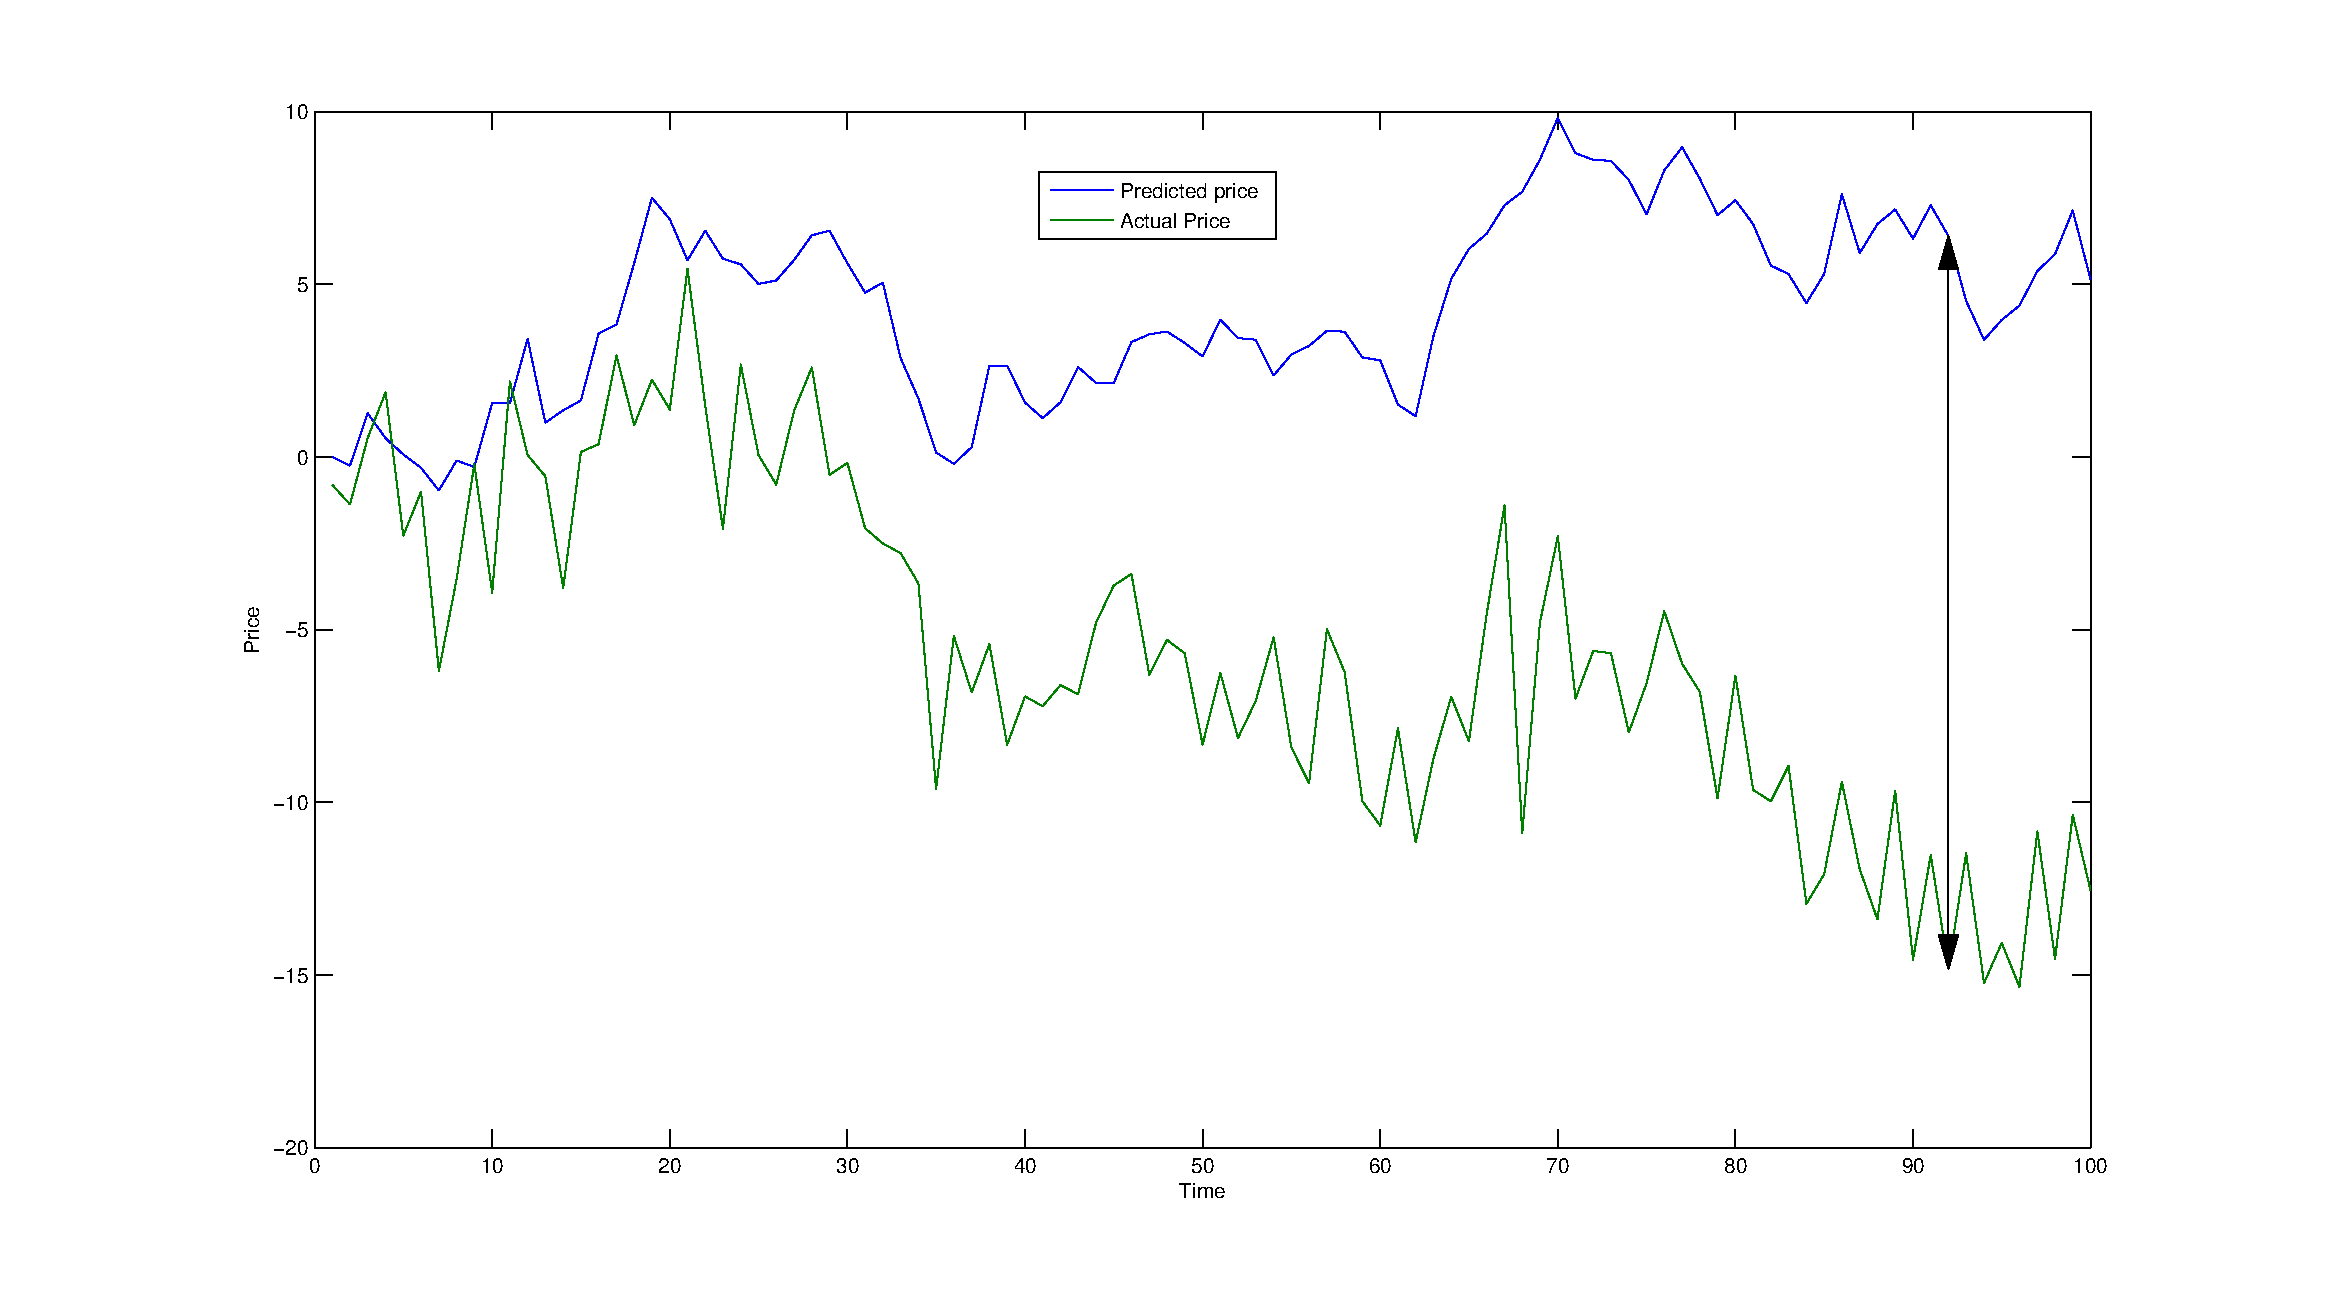
\includegraphics[scale=0.9]{mse.eps}

\end{center}
\caption{The arrow demonstrates the differences between the predicted price and the actual price in the test set that we hope to minimise.}
\end{figure*}


By carrying out the above procedure with different sets of test and training data we will be able to establish the predictive power of our model as well as determine how far into the future we will be able to make effective predictions. It is expected that the performance of the prediction will deteriorate for predictions further into the future as shown in the figure above.

If the system will be used for training than the complex regression problem can be reduced to a simpler classification problem. Instead of predicting the exact price we will instead classify whether stock is going to go up or down after a specific amount of time. When evaluating this approach we intend to use the number of misclassification as a metric for determining the predictive power of our algorithm.


\bigskip

\Subhead{Back-testing}

While mean square error in prediction is useful in evaluating algorithm effectiveness, low mean square error does not directly translate into trading performance.  

The simple price model will need be further extended to incorporate stock liquidity and ensure that gains can be realised. Further optimisation is possible by incorporating trading fees as well as liquidity rebates to ensure that the system not only maximises prediction power but also profitability.


\bigskip
\hrule
\end{textblock}


\begin{textblock}{7}(16,6.85)
\bigskip
\bigskip
\bigskip
\bigskip


\sf



\vspace*{4mm} % Sometimes you will have to fudge the final spacing.
\bigskip

\end{textblock}

%----------------------------------------------------------------------%
%            Construction lines                                        %

%\begin{textblock}{23}(0,2)\rule{\textwidth}{0.1mm}\end{textblock}
% Shows where the bottom of the header bar should fall.

%\begin{textblock}{23}(0,2.4)\rule{\textwidth}{0.1mm}\end{textblock}
% Shows where the top of each column should start.

%\begin{textblock}{23}(0,12)\rule{\textwidth}{0.1mm}\end{textblock}
% Shows where the bottom of the lowest block in each column should end

%\begin{textblock}{1.5}(6,4.12)\rule{\textwidth}{0.1mm}\end{textblock}
%\begin{textblock}{1.5}(6,4.52)\rule{\textwidth}{0.1mm}\end{textblock}
% Used to find the base of the first block and thus the top of the second.

%\begin{textblock}{1.5}(14,4.85)\rule{\textwidth}{0.1mm}\end{textblock}
%\begin{textblock}{1.5}(14,5.25)\rule{\textwidth}{0.1mm}\end{textblock}
% Same purpose but in the second column.

%\begin{textblock}{1.5}(15,6.05)\rule{\textwidth}{0.1mm}\end{textblock}
%\begin{textblock}{1.5}(15,6.45)\rule{\textwidth}{0.1mm}\end{textblock}
% Same purpose but in the third column.

\end{document}
